\subsection{Finite element modeling (\texttt{Fem})}
\label{sec:C5:fem}
Following the mesh generation process, \textit{Sorotoki} offers a nonlinear finite element solver for both quasi-static and fully dynamic simulations. An illustration of the FEM approach is given in Figure \ref{fig:C5:illustration_FEM}. FEM-based tools are crucial when describing large deformations in soft robots, which also accounts for hyperelastic materials and geometric nonlinearities. The FEM package is provided in a class called \class{Fem.m} and can be instantiated using \code{fem = Fem(Mesh)}. This class serves two main purposes: ($i$) to solve static or dynamic continuum problems with high accuracy, and ($ii$) to solve gradient-based optimization problems, also known as inverse design problems. It is important to note that, unlike \textit{SOFA}, the focus of \textit{Sorotoki} is on high-detail simulations rather than real-time implementation for control. The presented FEM simulation models are not intended for real-time applications, but rather for system identification and analysis.

\begin{figure}
\centering
%FemExample
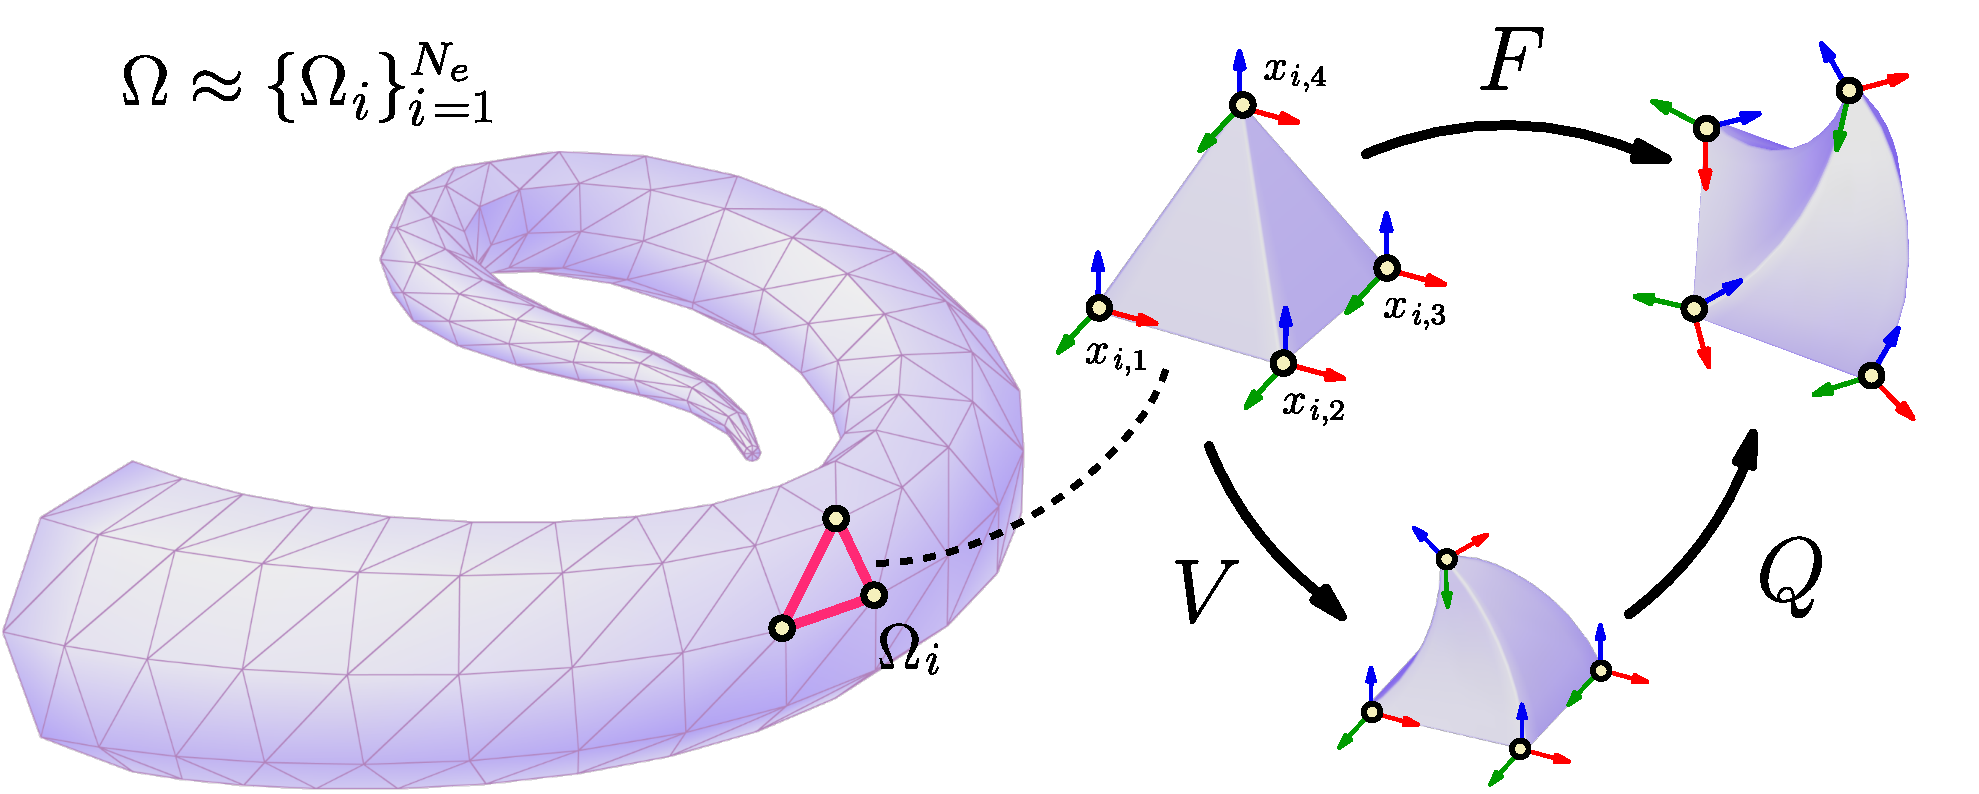
\includegraphics[width=0.85\textwidth]{./pdf/FemExample.pdf}
%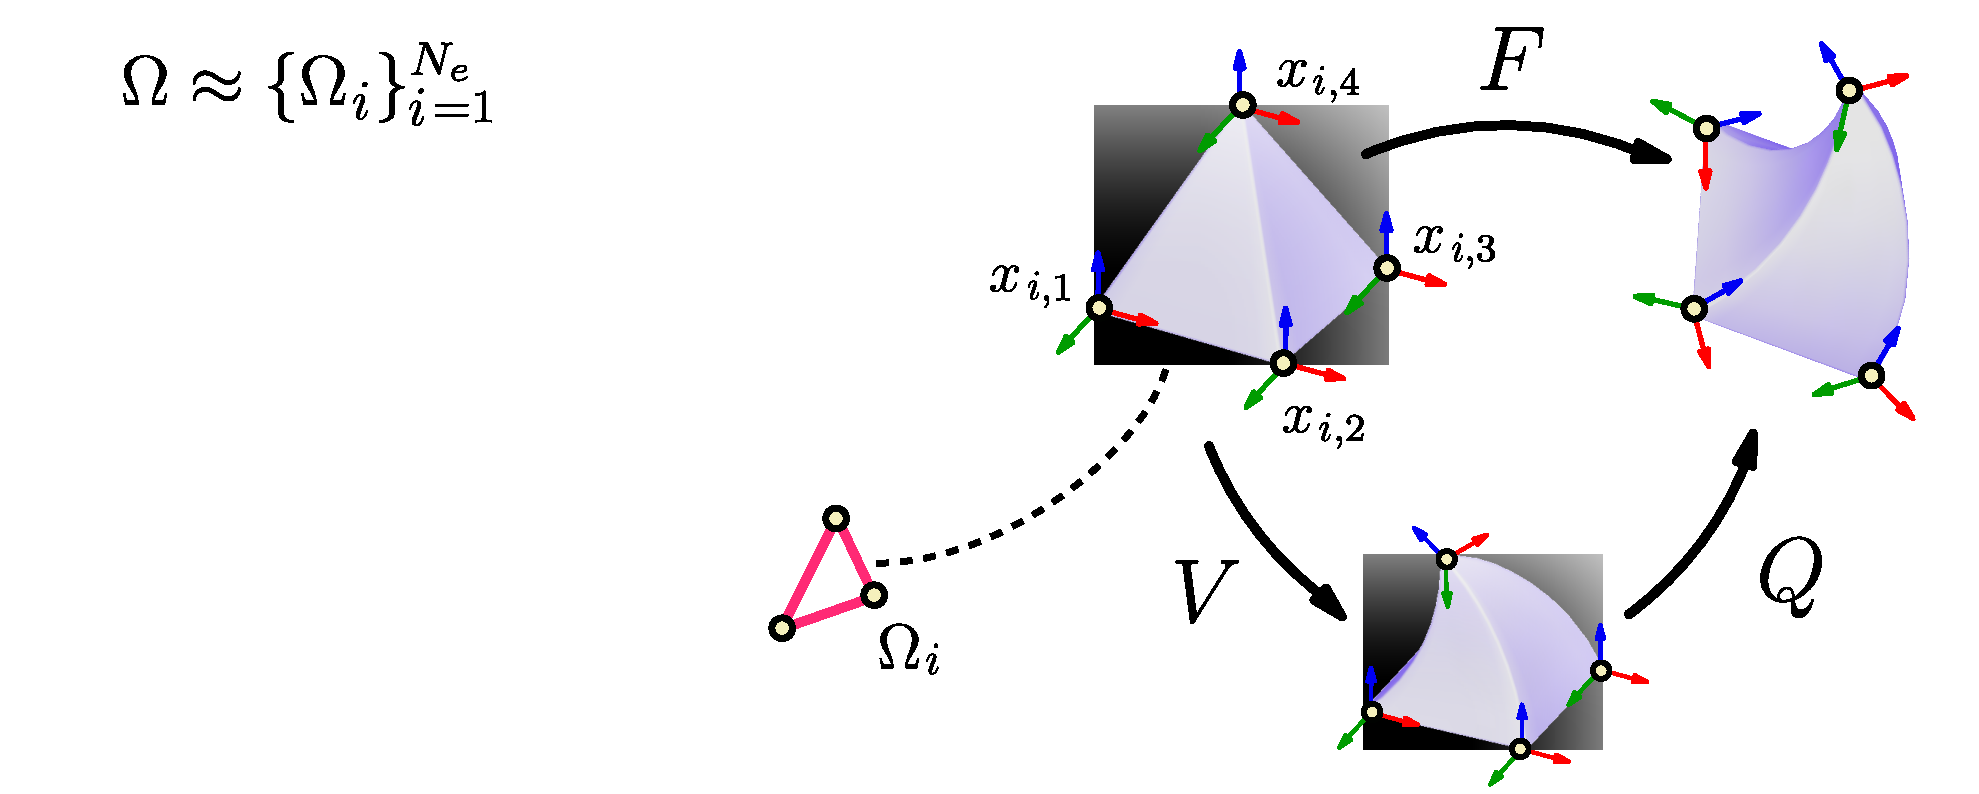
\includegraphics[width=0.85\textwidth]{./pdf/thesis-figure-6-5.pdf}
\caption{Illustration of the Finite Element Method (FEM), where a solid geometry $\Omega$ is subdivided into $N_e$ finite elements $\Omega_e$. Each element has $\dim(\x_e)$ DOFs, which allows the computation of the deformation gradient $\FB$. The deformation gradient can be decomposed into $\FB = \QB\VB$, an isochoric deformation part $\VB$ and rigid-body rotation part $\QB$. }    
\label{fig:C5:illustration_FEM}
\end{figure}

\textbf{A: High-detail finite element model.} The nonlinear dynamics of the finite element model in \textit{Sorotoki}, similar to \textit{SOFA} and \textit{Gibbon}, can be described by the general Newton-Euler equation of motion:
%
\begin{equation}
    \MB \ddx + \fB_\textrm{mat}(\x,\dx) + \fB\grav = \fB_{\textrm{u}}(\x,\uB,t) + \fB_{\Omega_{\textrm{env}}}(\x,\dx,t),
    \label{eq:C5:femmodel}
\end{equation}
%
where $\x$, $\dx$, and $\ddx$ are the global nodal displacement, velocities and accelerations of the mesh tesselation, respectively; $\MB$ the constant generalized mass matrix, $\fB_\textrm{mat}$ the internal soft material forces, $\fB_\textrm{g}$ the constant gravitational forces, $\fB_u$ a user-defined input, and $\fB_{\Omega_{\textrm{env}}}$ the normal reaction forces and tangent friction forces imposed by the dynamic contact with a (possibly time-dependent) environment $\Omega_{\textrm{env}}$. The environment $\Omega_{\textrm{env}}$ can be described using the SDF functionality (see Section \ref{sec:C5:sdf}) using the syntax \code{fem.addContact(sdf)}. A broad collection of generalized external inputs can be added using: \code{fem.addLoad}, \code{fem.addDisplace}, \code{fem.addGravity}, and \code{fem.addTendon}. Time-varying pressure inputs can be added using the command \code{fem.addPressure}. 

Without loss of generality, the material force can be decomposed into a position-dependent and velocity-dependent part: $\vec{f}_{\textrm{mat}}(\vec{x},\dot{\vec{x}}) = \vec{f}_{\textrm{e}}(\vec{x}) + \vec{f}_{\textrm{d}}(\dot{\vec{x}})$, \ie, an elastic and dissipation contribution, respectively. We assume that the dissipation is given by $\vec{f}_{\textrm{d}} = \zeta \mathbf{M} \dot{\vec{x}}$ with damping coefficient $\zeta > 0$. Materials can be assigned using \code{fem.addMaterial}. Note that the conservative elastic material forces $\vec{f}_{\textrm{e}}$ require more involved computation. Since this computation is not straightforward, we briefly explain the derivation of the nonlinear hyper-elastic material forces in \eqref{eq:C5:femmodel}, which follows standard nonlinear finite element procedures \cite{Kim2018,Holzapfel2002,Smith2018}. \\

\begin{intermez}[Deformation gradient]
\vspace{-3mm}
A fundamental measure of deformation in continuum mechanics is the deformation gradient, denoted by $\mathbf{F}$. The deformation gradient characterizes the local deformation for a neighborhood of the continuum body $\Omega$. Since a subvolume of the continuum body cannot be reduced to a point, it follows that $\det{\mathbf{F}} = J > 0$ and $\mathbf{F}^{-1}$ exists. The term $J$ is called the relative volume change and it is equal to 1 for isochoric deformations, such as rigid body deformations. Given these properties, the deformation gradient can then be factorized into $\mathbf{F} = \mathbf{Q} \mathbf{V}$, where $\mathbf{V} \succ 0$ is the right-handed stretch tensor and $\mathbf{Q} \in \mathrm{SO}(3)$ is a rotation matrix belonging to the special orthogonal group \cite{Holzapfel2002,Kim2018,Smith2018}. For convenience, we summarize the derived quantities of $\mathbf{F}$ in Table \ref{tab:C5:strain_measures} that will be used throughout this section. \\
\end{intermez}

\begin{table}
    \setlength{\tabcolsep}{2.25pt}
    %\rowcolors{1}{}{lightgray}
    \centering
    \caption{Table of deformations measures relevant for continuum mechanics problem. All measures can be related to the first-order deformation tensor $\FB$, following the works  \cite{Holzapfel2002,Kim2018,Smith2018}.}
    \label{tab:C5:strain_measures}
    \rowcolors{1}{}{blue!5}
    \begin{tabular}{ll}
        \hline
        Deformation measure       & \quad \; Derivation                                                     \\
        \hline \hline
        Relative volume change    & \quad \; $J = \det{\FB}$                                                \\
        Polar decomposition       & \quad \; $\FB = \QB \VB$                                                \\
        Right Cauchy-Green tensor & \quad \; $\CB = \FB^\top \FB$                                           \\
        First strain invariant    & \quad \; $I_1 = \trace(\CB)$,                                           \\
        Second strain invariant   & \quad \; $I_2 = \frac{1}{2}\left[ \trace(\CB)^2 - \trace(\CB^2)\right]$ \\
        First strain invariant    & \quad \;\ $I_3 = \det{\CB}$                                             \\
        \hline
    \end{tabular}
\end{table}
%
\begin{intermez}[Derivation of hyperelastic forces]
    
Let $\Omega_i$ denote the subspace spanned by the $i$-th element of the finite element mesh, and let $\x_i$ denote its nodal displacement vector. The elasticity of the constitutive soft material can be described by a strain-energy density function $\Psi: \FB \to \R_{\ge 0}$. A comprehensive discussion on common constitutive models for $\Psi$ will be provided later in the subsequent paragraph. The elastic potential energy of the continuum body is given by $\mathcal{U}_e = \int_\Omega \Psi(\cdot) \; dV$, and the conservative hyper-elastic force contribution can be computed as $\fB_e := \nabla_{\x}\,\mathcal{U}_e$. This contribution can be approximated using piecewise finite element interpolation and integrated using the Gauss quadrature rule \cite{Kim2018} as follows:
    %
    \begin{align}
        \fB_\textrm{e}(\x) & = \sum_{i=1}^{N_e} \frac{d}{d\x_i} \left\{\int_{\Omega_i} \Psi(\FB(\x_i,s)) \; ds\right\}, \notag                                                    \\
                           & \approx \sum_{i=1}^{N_e} \sum_{j=1}^{N_w} w_j \, \underbrace{\frac{\p \Psi}{\p \FB}(\FB(\x_i,s_j)) }_{\textrm{PK1}} \frac{\p \FB}{\p \x_i}(\x_i,s_j)
        \label{eq:C5:fem_hyper}
    \end{align}
    %
where the Gauss weights are denoted by $w_j > 0$, and the number of finite elements and Gauss samples are represented by $N_e$ and $N_w$, respectively.

The term $\frac{\partial \Psi}{\partial \FB}$ is also referred to as the first Piolla-Kirchhoff (PK1) stress tensor, which can be represented in closed-form for many constitutive models. The term $\frac{\partial \FB}{\partial \x_e}$ denotes the deformation Jacobian, which can also be given in closed-form but depends on the choice of element type. In addition to the first Piolla stress tensor, we also introduce the Cauchy stress tensor (i.e., true stress) $\vec{\sigma} := J^{-1} \frac{\partial \Psi}{\partial \FB} \FB^\top$, which is a symmetric second-order tensor whose components represent the true stress. It should be noted that these tensor calculations are highly nonlinear, making their computation the most time-consuming aspect of the finite element assembly. To enhance computational efficiency, the toolkit employs \texttt{.mex} executable code that is generated during installation (\texttt{Matlab Coder} toolkit is required).
\end{intermez}

%\subsubsection{Hyperelastic models and soft material presets}
%\label{sec:C5:hyperelastic}
\textbf{B: Hyperelastic models and soft material presets.} An important aspect of soft robotics in general is to accurately describe large nonlinear deformations of inertial continuum bodies in motion. Yet, due to these large deformations, many classical Hookean elasticity models may not be accurate for elastomer materials. 

To address this, \textit{Sorotoki} provides a library of hyper-elastic constitutive material models: Neo-Hookean (NH), Mooney-Rivlin (MR), and Yeoh model (YH). The strain energy densities for these models are derived based on the strain invariants $I_1$, $I_2$, and $I_3$ provided in Table \ref{tab:C5:strain_measures} and are shown in Table \ref{tab:C5:elasticitymodels}.
%
\begin{table}[t]
    \renewcommand\arraystretch{1.25}
    \setlength{\tabcolsep}{2.25pt}
    \rowcolors{1}{}{blue!5}
    %\rowcolors{1}{}{lightgray}
    \centering
    \caption{Table of material models included in \textit{Sorotoki}, including the NeoHookean model (NH), Mooney-Rivlin model (MR), and Yeoh (YH) model.}
    \label{tab:C5:elasticitymodels}
    \begin{tabular}{lcl}
        \hline
        Material model     & \;\;Parameters\;\; & \quad \;\; Energy-density potential $\Psi$                                     \\
        \hline \hline
        Neo-Hookean (NH)   & $(\mu)$            & \quad \;\; $\Psi_{\textrm{NH}} := \frac{\mu}{2} \left(I_1 - 3 \right)$         \\
        Mooney-Rivlin (MR) & $(c_1,c_2)$        & \quad \;\; $\Psi_{\textrm{MR}} := \sum^{2}_{i=1} c_i \left(I_i - 3 \right)$    \\
        Yeoh (YH)          & $(c_1,c_2,c_3)$    & \quad \;\; $\Psi_{\textrm{YH}}  := \sum^{3}_{i=1} c_i \left(I_1 - 3 \right)^i$ \\
        \hline
    \end{tabular}
\end{table}
%
The material models presented in Table \ref{tab:C5:elasticitymodels} are implemented in \textit{Sorotoki} under the class \class{Material}, but have specific constructors tailored towards each material, \texttt{NeoHookeanMaterial}, \texttt{MooneyMaterial}, and \texttt{YeohMaterial}. Regarding their parameters, the work of Marechal et al. \cite{Marechal2021Jun} provides an open-source database that includes a broad collection of soft materials commonly used in soft robotics, gathered through uniaxial material tests. Based on their dataset and relevant other literature \cite{Xavier2022Jun,Smith2018,Kim2018,Goury2018}, \textit{Sorotoki} offers some preset material models of soft materials commonly used in soft robotics, such as the Ecoflex30/50 series, Dragonskin10/30 series, NinjaFlex, and Formlabs Elastic50A/80A material. These material classes also include the physical data for density, viscosity, and tangential contact friction. Following \eqref{eq:C5:fem_hyper}, the first Piola-Kirchhoff (PK1) stress tensor is evaluated analytically using the function call \code{P = Material.PiollaStress(F)}.  \\
%

\textbf{C: Finite element solvers and (nonlinear) modal analysis}
To solve the structural forward dynamics of the system \eqref{eq:C5:femmodel}, the toolkit uses an implicit Newmark-$\beta$ solver \cite{Newmark1959Jul}, which is briefly outlined in Appendix \ref{app:C5:newmark}. Implicit solvers offer improved stability compared to explicit methods, such as the Runge-Kutta solver (\texttt{ode45}), particularly when larger time steps are employed. However, the cost of larger time steps is a decreased numerical precision.  Alternatively, for quasi-static problems when $\ddx = \dx = \vec{0}_n$, we aim to seek the solutions to the static force equilibrium $\rB(\x) = \vec{0}_n$ where $\rB := -\fB_{\textrm{mat}} + \fB\grav + \fB_\textrm{u} + \fB_{\Omega_{\textrm{env}}}$ is the force residual vector. The nonlinear equality for nodal displacements $\x$ is solved using an iterative Newton-Raphson solver. To call these solvers, dynamic simulations are executed with \code{fem.simulate()} and quasi-static simulations with \code{fem.solve()}. Upon completion of a simulation, all displacements, velocities, forces, and stress information are stored in the \code{fem.Log} data structure. This log file can be accessed for data analysis or during simulation to facilitate state feedback control.

Alternatively, we can explore nonlinear modal analysis at any quasi-static equilibrium configuration $\x^* \in \mathcal{X}$ of the system \eqref{eq:C5:femmodel}. Let $\KB_T:= \left[\frac{\p \fB\elastic}{\p x_1} \;\hdots\; \frac{\p \fB\elastic}{\p x_2} \right]$ be the Jacobian matrix of the (nonlinear) elastic potential forces, also referred to as the tangent stiffness. Then, the local eigenvalue problem for the linearized FEM model around the point $\x^*$ is given by 
%
\begin{equation}
\Big[\KB_T(\x^*)- \lambda_i \MB \Big] \thetaB_i = \vec{0}_n,
\label{eq:C5:eigenmode_decomposition}
\end{equation}
%
where $\lambda_i$ is a real scalar eigenvalue and $\thetaB_i$ is its corresponding eigenmode. The dynamic analysis is implemented in Sorotoki using \code{fem = fem.analysis(x)}, which stores the necessary data in \code{fem.Log}. It is important to note that, unlike linear finite element models, the set of eigenmodes ${\thetaB_i}$ obtained from the eigenvalue decomposition in \eqref{eq:C5:eigenmode_decomposition} is highly dependent on the linearization point $\x^*$ and may thus not be unique for all $\x^* \in \mathcal{X}$.

\begin{example}[Nonlinear buckling analysis via decomposition]
%\subsubsection*{Example C1: Nonlinear buckling analysis via decomposition}
An excellent case study of the eigenvalue problem in nonlinear elasticity systems is the buckling behavior of patterned elastomer metamaterials, as studied by Bertoldi et al. \cite{Bertoldi2008} and later by Overvelde et al. \cite{Overvelde2012May}. In their studies, an elastomer specimen with a periodic circular porous structure was subjected to uniaxial compression. The specimen displayed an inward buckling phenomenon at a critical loading point, resulting in the specimen exhibiting a negative Poisson ratio, \ie, auxetic behavior. To be specific, the structure undergoes a so-called "bifurcation" where solutions switch stability or new solutions arise for a critical parameter value. In this case, the bifurcation parameter is the compression ratio $\varepsilon$.

In accordance with \cite{Overvelde2012May}, a square elastomer specimen with circular holes was modeled using a Neo-Hookean material model, with Young's modulus $E = 19$ (\si{\kilo \pascal}) and Poisson ratio $\nu = 0.45$. As reported in \cite{Overvelde2012May}, the critical buckling point was observed to occur at approximately $\varepsilon = -12.5\%$ uniaxial compression.

\begin{figure}[!t]
    \centering
\includegraphics*[width=0.95\textwidth]{./pdf/thesis-figure-6-6-1.pdf} \\[0.5em]
\includegraphics*[width=0.95\textwidth]{./pdf/thesis-figure-6-6-2.pdf}
    %\input{./fig/fig_bucklemode_linear.tex}
%\input{./fig/fig_bucklemode_nonlinear.tex}
\caption{Nonlinear buckling mode analysis of periodic circular porous elastic structure inspired by \cite{Bertoldi2008,Overvelde2012May}. The horizontal displacements are indicated by \protect\colormapcaption{0}{.75cm}$\!\!\in [-5,5]$ \si{\milli \meter}. (top) The first four eigenmodes of the elastomer structure for $\varepsilon = 0\%$ compression, no buckling modes appear. (bottom)  The first four eigenmodes for $\varepsilon = 12.5\%$ compression. Notice that the first mode $\thetaB_1$ is a buckling mode where the collapses holes orient periodically either vertically or horizontally. }
\label{fig:C5:fig_bucklemode}
\vspace{-3mm}
\end{figure}

A numerical solution is obtained through quasi-static analysis using the function \code{fem.solve}. To model compression, a displacement load was added using \code{fem.addDisplace('Top')}. The resulting equilibrium configuration was then utilized in the eigenvalue problem via the function \code{fem.analysis(x)}. The eigenmodes for the zero-stress and $\varepsilon = -12.5\%$ compression cases are illustrated in Figure \ref{fig:C5:fig_bucklemode}. It is worth noting that the first three eigenmodes of the elastomer structure at $\varepsilon = 0\%$ compression exhibit no buckling modes. Conversely, the first eigenmode $\thetaB_1$ at $\varepsilon = -12.5\%$ compression displays a buckling mode, wherein the collapse of the holes is periodically oriented either vertically or horizontally. This buckling mode is in accordance with the experiments from \cite{Overvelde2012May} and \cite{Bertoldi2008}. The supplementary code is provided below: 
\end{example}
%

\begin{matlabcode}
%% EXAMPLE: Fem class 
load('sdf_porous_square.mat');
msh = Mesh(sdf, 'NElem', 5e3);
fem = Fem(msh, 'TimeStep', 1/60);

% assign material 
fem.Material = NeoHookeanMaterial(1.0, 0.45);

% add displacement and forces 
fem = fem.addConstraint('Bottom', [1,1]);
fem = fem.addConstraint('Top', [1,0]);
fem = fem.addDisplace('Top', [0,-0.125 * W]);

%  quasi-solve and eigen-analysis 
fem = fem.solve();
fem = fem.analysis( fem.Log.x(:,end) );
\end{matlabcode}
    

\begin{example}[Locomotion dynamics of soft crawling robot]
To demonstrate a dynamic finite element method (FEM) simulation that incorporates contact, we will utilize \sorotoki to model the locomotion of a multi-gait soft robot crawler inspired by the work of Shepard \cite{Shepherd2011Dec}. The study by Shepard  et al. \cite{Shepherd2011Dec} presents a soft robot system that consists of five pressure chambers - four for each leg and one for the spine. The pressure chambers are actuated in a sequential manner to produce an undulating motion. The work of Shepard  et al. \cite{Shepherd2011Dec} demonstrates that complex locomotion can be achieved through the use of open-loop controllers and the dynamic interaction between the soft robot and its environment.

To simplify the model, we assume general plane motion. The geometry of the soft crawler's cross-section is first provided to \texttt{Mesh.m} to generate a triangular mesh. Then, a finite element method (FEM) model is generated, with the material model \texttt{fem.Material = Ecoflex0030}. To model the environment, the function \texttt{fem = fem.addContact(sLine)} is utilized, which simply creates an unbounded horizontal line. In accordance with \cite{Shepherd2011Dec}, a harmonic excitation is applied to each chamber, as expressed by the following: $u_i = A\cdot\textrm{sat}\left[\sin(\omega t - \phi_i) \right]$, where the index $i \in {1,2,3}$ represents the front, middle, and back pressure chambers embedded in the soft body. 

\begin{matlabcode} 
%% EXAMPLE: Fem class   
msh = Mesh('MultiGait.png', 'MeshSize', 1.0, ...
            'BdBox', [0, 150, 0, 12]);

% -- mesh to fem 
fem = Fem(msh,'TimeStep',1/500);
fem.Material = Ecoflex50();

% -- add inextensible bottom layer 
E1  = fem.findElements([0 150 0 2]);
fem = fem.addMaterialModifier(E1, 5);

% -- add forces and constraints 
Y  = 'BoxSelect';
C1 = fem.findEdges(Y,[0   50 0 15]);
C2 = fem.findEdges(Y,[50  100 0 15]);
C3 = fem.findEdges(Y,[100 150 0 15]);

fem = fem.addPressure(C1, @(x) Pressure(x,1));
fem = fem.addPressure(C2, @(x) Pressure(x,2));
fem = fem.addPressure(C3, @(x) Pressure(x,3));

fem = fem.addGravity();
fem = fem.addContact(sLine());

% -- solve dynamics 
fem = fem.simulate();

% -- open-loop controller 
function y = Pressure(fem, i)
    phi = pi / 3 * (i - 1);
    y = clamp(sin(5*pi*fem.Log.t - phi), 0, Inf);
end
\end{matlabcode}
\vfill
The excitation signal parameters are set as follows: $A = 45$ \si{\kilo \pascal}, $\omega = 5 \pi$ \si{\radian}, and $\phi_i = \frac{\pi}{3} \cdot (i-1)$ \si{\radian}. The saturation function is defined as $\textrm{sat}(x) = 0$ for $x < 0$, and $\textrm{sat}(x) = x$ for $x \geq 0$. Gravitational acceleration is added, and the dynamic simulation solver is invoked using \texttt{fem.simulate}. Figure \ref{fig:C5:fem_example_crawl} presents a comparison between the soft robot described in \cite{Shepherd2011Dec} and the dynamic simulation performed by \texttt{Sorotoki}.

The results of the simulation performed using \textit{Sorotoki} show a morphological behavior that is consistent with the experimental recordings. Figure \ref{fig:C5:fem_example_crawl_com} depicts the trajectory of the center of mass (CoM) of the soft robot during the undulating locomotion. Note that an identical stair-like evolution of the CoM is also observed in the work of Shepard et al. \cite{Shepherd2011Dec}. 
\vfill
\end{example}

% \begin{figure}
% %\includegraphics[width=0.485\textwidth]{./fig/PipelineCrawler.pdf}
% \caption{Overview of the software pipeline showing the interconnected classes required to simulate the soft crawler with environmental contact.}    
% \label{fig:C5:PipelineCrawler}
% \vspace{-5mm}
% \end{figure}
%

\afterpage{
\begin{sidewaysfigure*}[t]
\vspace{-5mm}
\centering
\includegraphics*[width=\textwidth]{./pdf/thesis-figure-6-8-1.pdf}
\includegraphics*[width=\textwidth]{./pdf/thesis-figure-6-8-2.pdf}
%\input{./fig/fig_fem_example_crawl_true.tex}
%\input{./fig/fig_fem_example_crawl.tex}
\caption{(top) Experiment of soft multi-gait crawling soft robot developed by Shepard et al \cite{Shepherd2011Dec} performing an undulating forward motion by periodic pressurizarion of its internal pressure chambers, back legs $\to$ middle $\to$ front legs. The soft robot is made from an elastomer material with strain-inhibit layer at the bottom to enhance bending. The Von Mises stresses are shown as \protect\colormapcaption{0}{.75cm}$\!\!\in [0,10]$ \si{\mega \pascal}. (bottom) Simulation recreation of the experiments performed by Shepard et al \cite{Shepherd2011Dec} using the Finite Element solver in the \sorotoki toolkit. Images sourced from public resources, with intellectual property belonging to cited authors, sources, and publishers. }
\label{fig:C5:fem_example_crawl} 
\vspace{5mm}
\includegraphics*[width=0.85\textwidth]{./pdf/thesis-figure-6-9-1a.pdf} 
%\includegraphics*[width=0.85\textwidth]{./pdf/thesis-figure-6-9-2a.pdf}
\caption{(top) Numerical simulation of the center of mass displacement and gait for undulating soft crawler. The horizontal displacement is given by \data{Matlab1}, and the vertical displacement as \data{Matlab2}. (bottom) The gait cycle of the soft crawler where the sequence $\{$\ldata{Matlab1}, \ldata{Matlab2}, \ldata{Matlab3}$\}$ shows the fluidic activation. }
\label{fig:C5:fem_example_crawl_com}
%\vspace{-5mm}
\end{sidewaysfigure*}
\clearpage
}

\textbf{Gradient-based computational (inverse) design}
Besides modeling, the field of computational inverse design can also benefit from the use of FEM models. Building up the \class{Fem} class, the objective is to find a topological structure of a continuum system based on a desired deformations or compliance. One widely adopted method is the Solid Isotropic Material with Penalization (SIMP) approach, which is a commonly used material interpolation technique in topology optimization \cite{Bendsoe2003}. In the SIMP method, each finite element $e \in \{1,2,...,n_e \}$ is assigned a continuous density variable $\rho_e \in (0,1]$, which serves as an indicator of the material distribution within the mesh. If $\rho_e = 1$, the element is considered solid, while if $\rho_e = 0$, the element is considered void. This assignment of density variables enables the modification of the strain energy density in \eqref{eq:C5:fem_hyper}:
%
\begin{equation}
\tilde{\Psi}_{e} = \left[ \varepsilon + (1-\varepsilon){\rho_e}^p \right] \Psi,
\end{equation}
%
where $0 < \varepsilon \ll 1$ a lower bound on the densities, and $p > 1$ a penalty factor for penalizing intermediate densities during the optimization process. By collecting the density values $\vec{\rho} = \textrm{col}\{\rho_1,\rho_2,...,\rho_{N_e}\}$, the inverse design problem can be formulated in terms of two unknowns: the displacement field $\xB$ and the density field $\vec{\rho}$. Consequently, the computational design problem for general soft material structures can be expressed as a nonlinear topology optimization problem of the following form:
%
\begin{mini}[2]
    {\vec{\rho}}{\Phi = -\beta_1\, \LB^\top\!\x \;+\; \beta_2 \fB\elastic^\top \! \fB_{\textrm{u}} }{}{}
    \addConstraint{\tilde{\rB}(\xB,\vec{\rho})=0,}{}{}
    \addConstraint{\vec{v}^\top \vec{\rho}\le v^\star,}{}{}
    \addConstraint{\vec{\rho}\in \mathcal{P},}{}{}
    \label{eq:C5:topo_optimization}
\end{mini}
%
where $\LB$ a sparse unit-vector composed of nonzero entries for the degrees-of-freedom corresponding to the desired morphology of the soft robot, $\vB$ the element volumes, $v*$ the desired volume infill, $\mathcal{P} = \left\{ \vec{\rho} \in \R^{n_e} ~|~  0 < \rho_i \le 1\right\}$ admissible set for the design variables, and $\beta_1$ and $\beta_2$ are positive scalars that can be adjusted to vary the optimization problem, with $\beta_1 \ll \beta_2$ resulting in compliance minimization and $\beta_1 \gg \beta_2$ leading to a compliant mechanism. To solve the optimization problem in Equation \eqref{eq:C5:topo_optimization}, we utilize the Method of Mixed Asymptotes (MMA) proposed by Svanberg \cite{Svanberg1987Feb,Svanberg2007}. Earlier work on this computational design approach was presented in Chapter \ref{chap: design}, and the chapter is referred to this work for the analytic gradients required for the MMA solver.

The optimization routine in the \textit{Sorotoki} framework is incorporated into the \code{Fem} class and can be invoked by utilizing the command \code{fem.optimize('type')}, where \code{'type'} represents the optimization problem at hand. For minimizing compliance, the cost function is self-adjoint \cite{Bendsoe2003}, hence objective function and constraints are linear operators. However, when dealing with compliant mechanisms, it is necessary to specify the selection vector $\LB$, which can be defined using the \code{fem.addOutput(id)} command. The value of \code{id} represents the nodal indices of interest, which can be identified using the \code{fem.Mesh.findNode} functionality.


